% Create a Table of Contents in Beamer
\documentclass[10pt,t]{beamer}
% Theme choice:
\usetheme{Singapore}
\useoutertheme{sidebar}
\usecolortheme{seahorse}
\setbeamercolor{titlelike}{bg=white}
\setbeamercolor{frametitle}{bg=white}
%\setbeamertemplate{frametitle}[default][left]
\setbeamertemplate{navigation symbols}{}

\usepackage{graphicx}
\usepackage{amsmath}
\usepackage{amsfonts}
\usepackage{amssymb}
\usepackage{amsthm}
\usepackage{ulem}
\usepackage{listings}
\usepackage{xcolor}
\usepackage{wrapfig}
\usepackage{subfig}
\usepackage{setspace}
\usepackage{enumerate}
\usepackage{verbatim}
\usepackage{tikz}

% new amber color
\definecolor{amber}{rgb}{1.0, 0.75, 0.0}

% Title page details: 
\title{Covariate adjustment in clinical trials} 
\author{Charlie Wolock}
\date{\today}


\begin{document}
	% Title page frame
\begin{frame}
	\titlepage 
\end{frame}


% Outline frame
\begin{frame}{Outline}
	\tableofcontents
\end{frame}

\AtBeginSection[ ]
{
	\begin{frame}{Outline}
		\tableofcontents[currentsection]
	\end{frame}
}


\section{Clinical trials}

\begin{frame}{What are clinical trials?}
	Clinical trials are studies performed in clinical research to evaluate biomedical or behavorial interventions (e.g. vaccines, drugs, medical devices). They are usually
	\begin{itemize}
		\item Prospective
		\item Reliant on human subjects
		\item Randomized: treatment assignment is random
		\item Controlled: there is a control group that receives no intervention (or a placebo) that serves as a comparator to the group receiving the intervention 
	\end{itemize}
	Statisticians often focus on the ability of clinical trials to provide information on efficacy, but safety is just as important!
	\begin{itemize}
		\item The FDA requires clinical trials for new products to ensure both of these criteria are met
	\end{itemize}
\end{frame}

\begin{frame}{Randomization and controls}
	The specific characteristics of RCTs that we'll focus on are
	\begin{itemize}
		\item Randomization: predictor of interest (treatment) is independent of all other covariates by design - confounding is not (theoretically) possible
		\item Controls: The presence of a control group allows us to make comparisons. We can imagine what might have happened to the treatment group had they not received treatment. 
	\end{itemize}
\begin{center}
	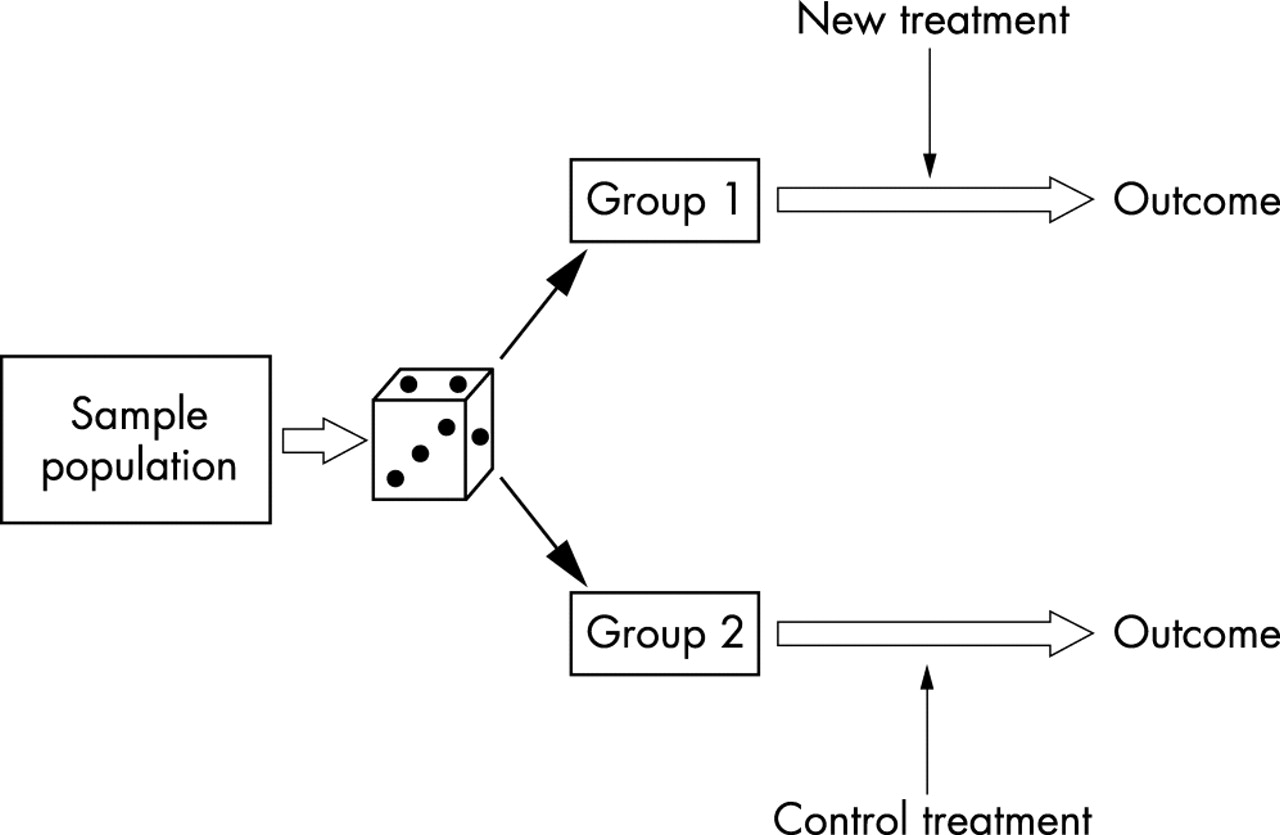
\includegraphics[width = 0.6\textwidth]{rct.jpg}
\end{center}
\end{frame}

\begin{frame}{Downsides of RCTs}
	\vspace{-0.8cm}
	\begin{itemize}
		\item Cost/time: Massively expensive to enroll hundreds or thousands of participants, can last for years
		\begin{center}
			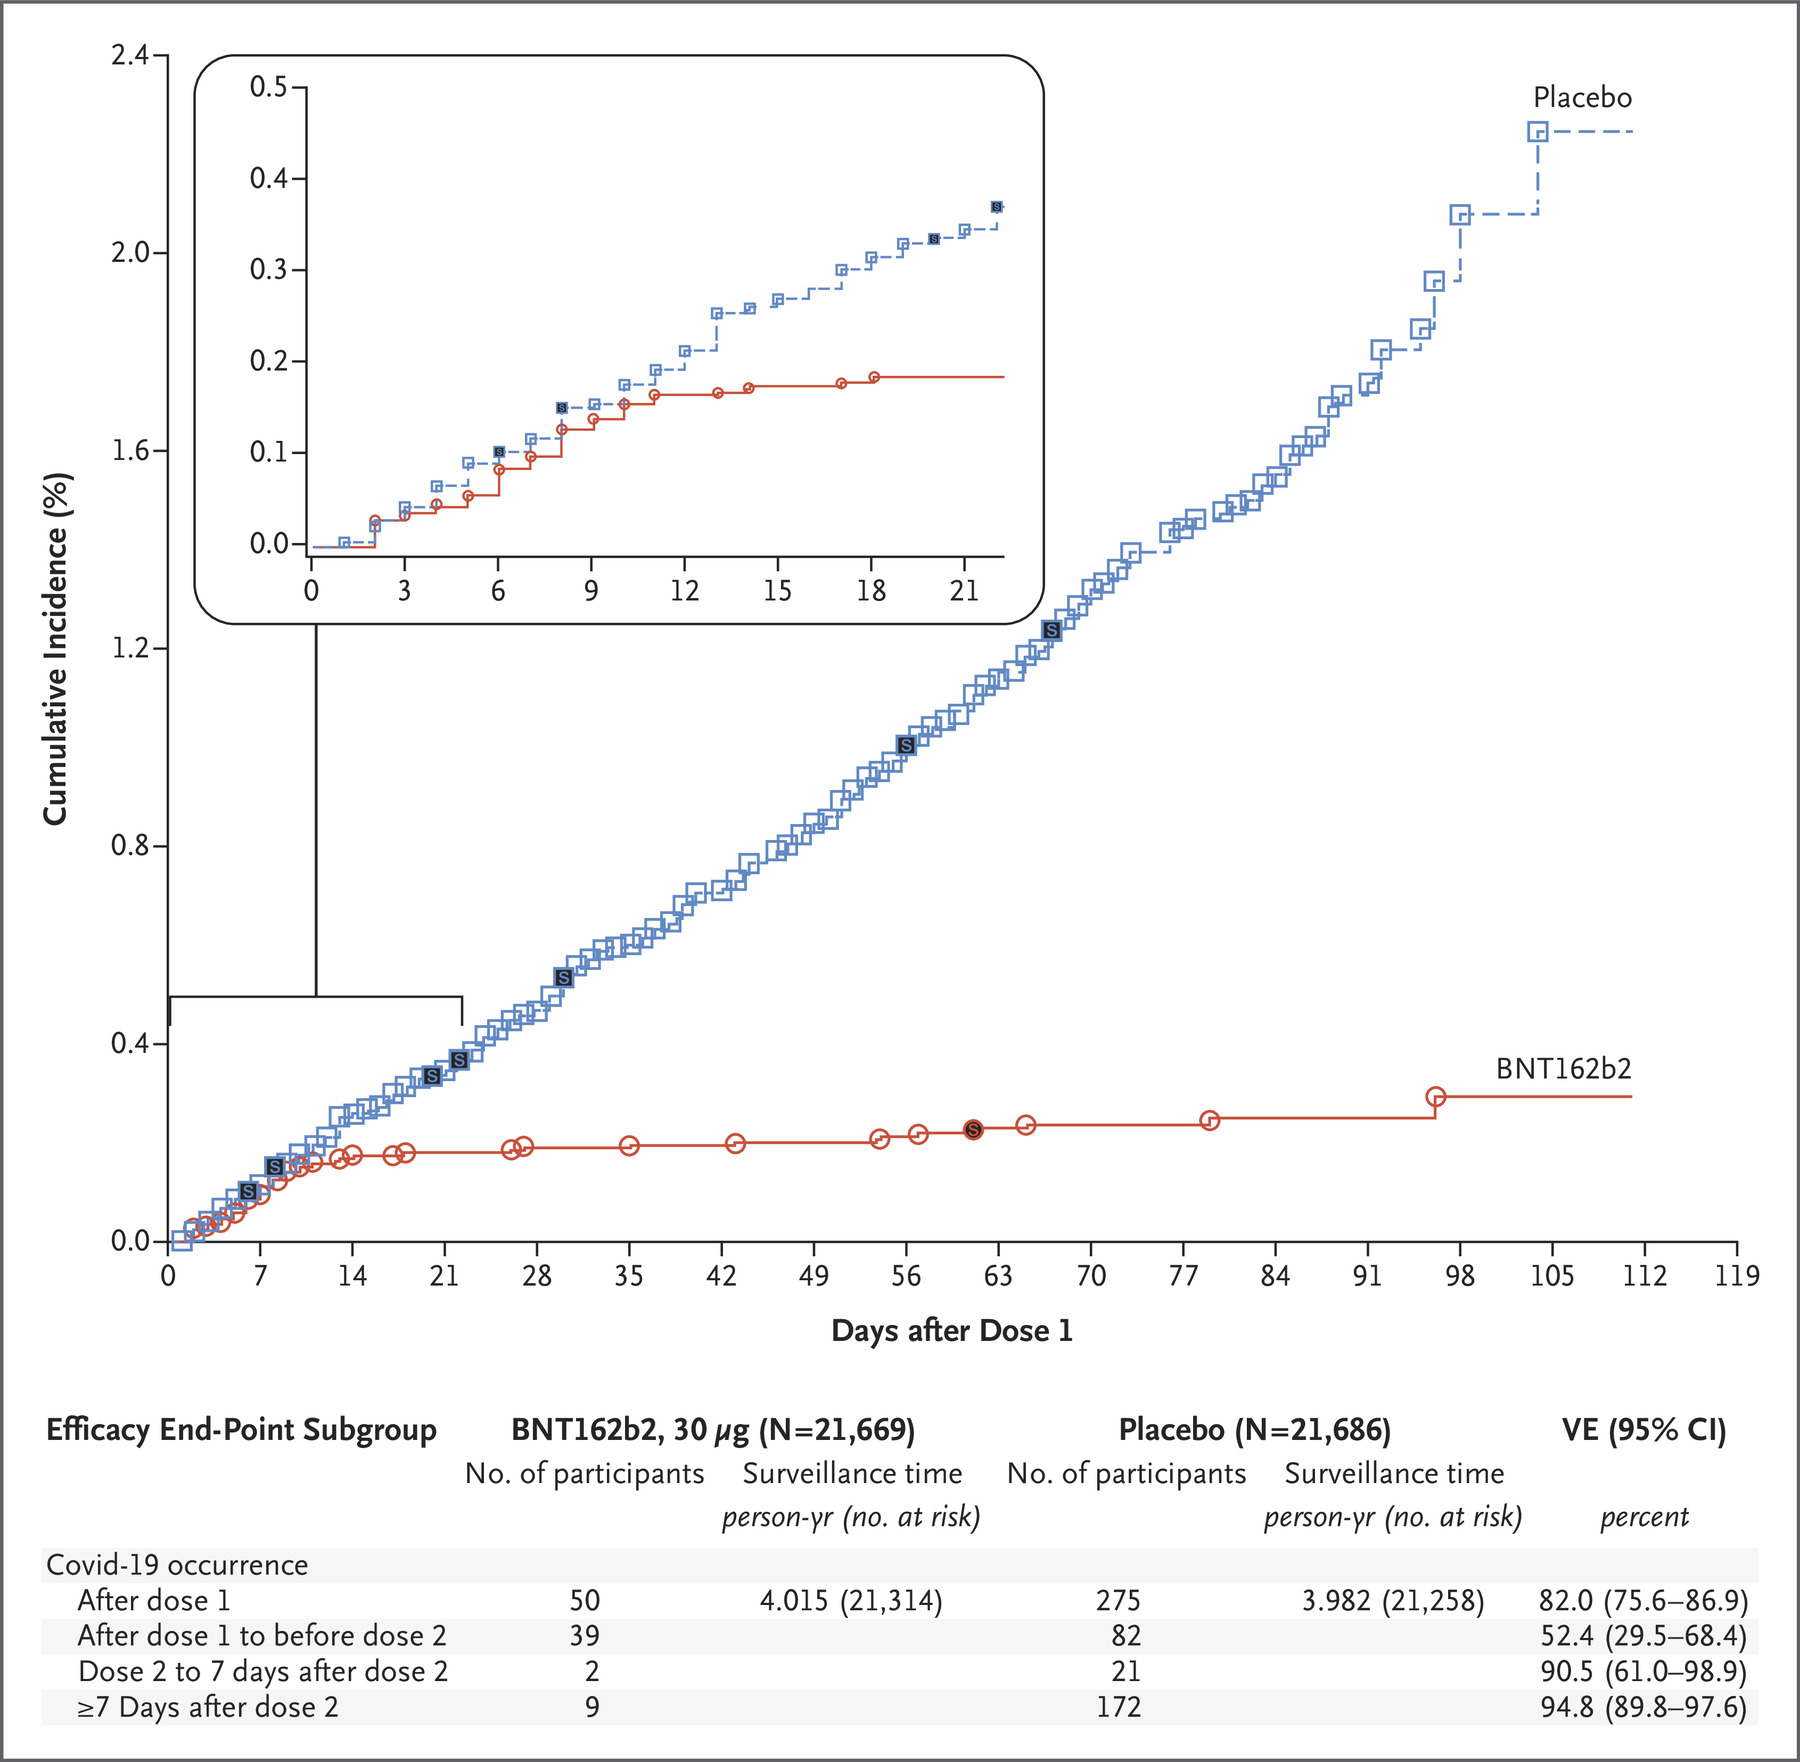
\includegraphics[width = 0.7\textwidth]{pfizer.jpeg}
		\end{center}
	\end{itemize}
\end{frame}

\begin{frame}{Downsides of RCTs}
	\begin{itemize}
		\item Ethics: If you have good reason to believe treatment is superior (or inferior) to placebo, is it ethical to randomize people to both groups?
		\begin{itemize}
			\item Clinical equipoise: There must be genuine uncertainty regarding which treatment is superior
		\end{itemize}
	\end{itemize}
\end{frame}

\begin{frame}{Motivation for efficiency}
	A major active question in biostatistics is
	\begin{itemize}
		\item Can we run smaller, shorter trials while still getting good estimates of treatment effect?
	\end{itemize}
	This brings us to the idea of statistical efficiency. 
\end{frame}

\section{Covariate adjustment}

\begin{frame}{Estimand of interest}
	Suppose in our trial we have a binary treatment $A$ (1 = treatment, 0 = placebo) and a quantitative outcome $Y$. We want to estimate (and do statistical inference on) the so-called ``average treatment effect" 
	\begin{align*}
		E[Y \mid A = 1] - E[Y \mid A = 0]
	\end{align*}
	\textbf{Question:} How would you estimate $E[Y \mid A = 1]$ and $E[Y \mid A = 0]$?\pause 
	\\ ~\ 
	
	\textbf{Answer:} Calculate sample average of $Y$ among those in the treatment group and among those in the control group, and take the difference!
	\begin{itemize}
		\item We will call this the unadjusted estimator, and label it $\hat{\theta}_1$. 
	\end{itemize}
\end{frame}

\begin{frame}{Estimator variance}
	As you probably intuited, $\hat{\theta}_1$ is unbiased for the true average treatment effect. In that sense, it's a good estimator. 
	\\ ~\ 
	
	But is this estimator efficient, in the sense that it makes good use of the data we have? 
	\\ ~\ 
	
	The variance of an estimator answers this question. For a given sample size, a smaller variance means a narrower confidence interval
	\begin{align*}
		\left(\hat{\theta}_1 - 1.96\times \frac{\sqrt{\text{Var}(\hat{\theta}_1)}}{\sqrt{n}}, \hat{\theta}_1 + 1.96\times \frac{\sqrt{\text{Var}(\hat{\theta}_1)}}{\sqrt{n}}\right)
	\end{align*} 
\end{frame}

\begin{frame}{Efficiency}
	Confidence interval width is key!
	\begin{itemize}
		\item For example, FDA approval of a COVID-19 vaccine required that the lower confidence interval bound for vaccine efficacy be above 30\%. 
		\begin{itemize}
			\item For a given point estimate, a wider confidence interval means we are less likely to be above that 30\% mark
		\end{itemize}
	\end{itemize}
	Two ways of thinking about efficiency:
	\begin{enumerate}
		\item For a fixed $n$, we can try to find an estimator with lower variance, and thereby get a narrower confidence interval
		\item For a fixed confidence interval width, finding an estimator with lower variance will allow us to use a smaller $n$
	\end{enumerate}
	Getting the same interval width with a smaller sample size is good!
	\begin{itemize}
		\item Save money
		\item Get effective treatments approved faster
		\item Avoid randomizing people to ineffective treatments
	\end{itemize}
\end{frame}

\begin{frame}{Covariate adjustment}
	\vspace{-0.8cm}
	\begin{center}
		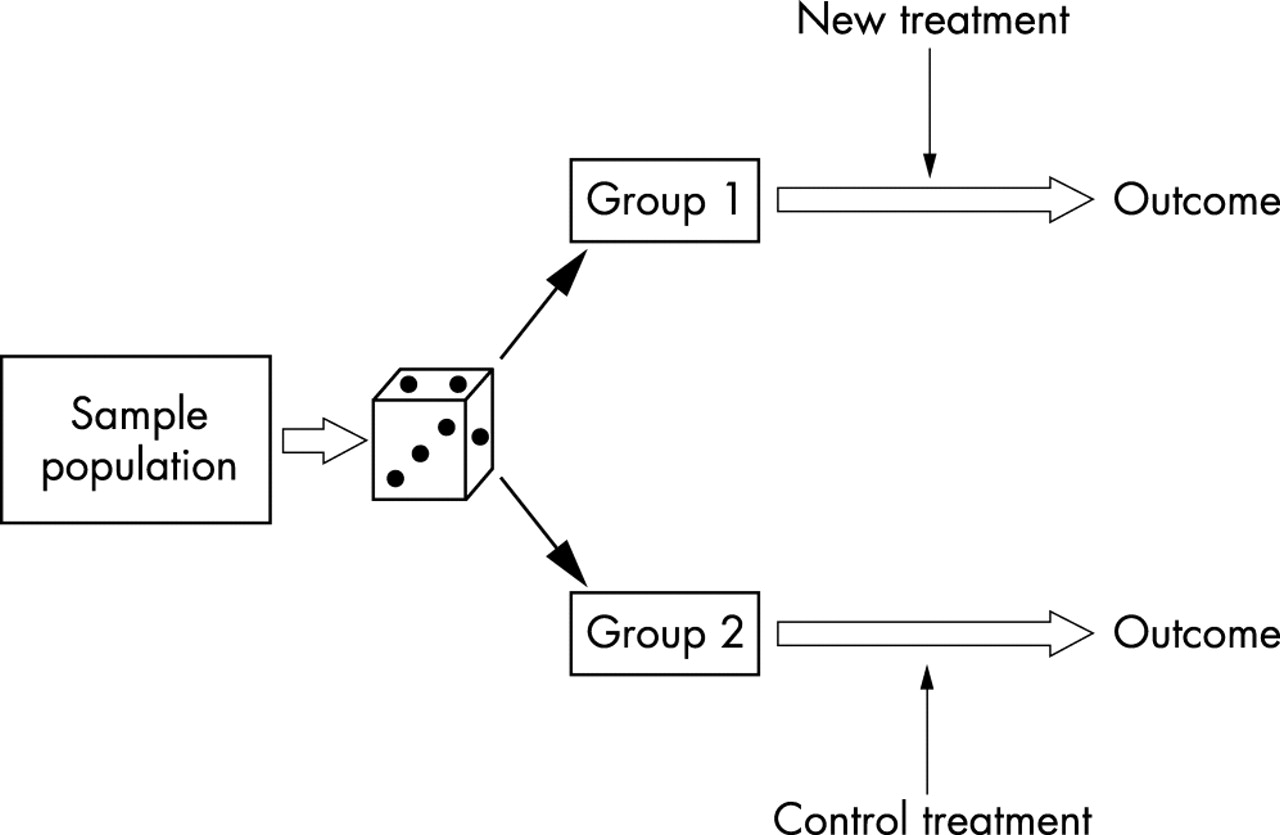
\includegraphics[width = 0.6\textwidth]{rct.jpg}
	\end{center}
	The approach where we separately estimate means in the two groups should remind you of a simple linear regression from Chapter 1. 
	\begin{align*}
		E[Y \mid A ] = \gamma_0 + \gamma_1 A
	\end{align*} 
\end{frame}

\begin{frame}{Covariate adjustment via outcome regression}
	Suppose that, in addition to $A$ and $Y$, we also measure a covariate $X$ that we think causally affects $Y$ (a precision variable). Consider the linear regression model
	\begin{align*}
		E[Y \mid A, X] = \beta_0 + \beta_1 A + \beta_2 X
	\end{align*}
	The usual interpretation of $\beta_1$ in this model is ``the average difference in $Y$ comparing treatment and placebo groups, for those with the same value of $X$." Using symbols:
	\begin{align*}
		E[Y \mid A = 1, X = x] - E[Y \mid A = 0, X = x]
	\end{align*}
	However, it turns out that, because $A$ and $X$ are independent by randomization, we can actually interpret $\beta_1$ as
	\begin{align*}
		E[Y \mid A = 1] - E[Y \mid A = 0],
	\end{align*}
	the average treatment effect!
\end{frame}

\begin{frame}{Covariate adjustment via outcome regression}
	This result actually holds \textcolor{blue}{whether or not the linearity assumption is met}. In other words, even if our linear model is misspecified, $\beta_1$ has the interpretation we want. 
	\begin{itemize}
		\item Remember, this is only true because we are dealing with RCTs!
	\end{itemize}
	This is known as the ANCOVA (analysis of covariance) estimator of the average treatment effect. 
	\\ ~\ 
	
	It can be shown that the variance of the ANCOVA estimator $\hat{\beta}_1$ is no larger than the variance of $\hat{\theta}_1$, and is generally smaller.
	\begin{align*}
		\text{Var}(\hat{\beta}_1) \leq \text{Var}(\hat{\theta}_1)
	\end{align*} 
	So ANCOVA is more efficient!
\end{frame}

\begin{frame}{Covariate adjustment via randomization probability}
	Including covariates in a linear regression for our outcome $Y$ is only one of the many ways to increase efficiency in a trial. 
	\\ ~\ 
	
	In a simple randomization scheme, we know that $P(A = 1) = 0.5$, independent of $X$. 
	\\ ~\ 
	
	But we might consider fitting a logistic regression
	\begin{align*}
		\log(\text{odds}(A = 1 \mid X)) = \phi_0 + \phi_1 X
	\end{align*}
	Let $\hat{g}(x) = \text{expit}(\hat{\phi}_0 + \hat{\phi}_1x)$ be the estimated probability of treatment for a subject with $X = x$. 
\end{frame}

\begin{frame}{Covariate adjustment via randomization probability}
	\vspace{-0.5cm}
	Instead of estimating $E[Y \mid A = 1]$ using the sample mean among the treated:
	\begin{align*}
		\frac{\frac{1}{n}\sum_{i=1}^{n}A_i Y_i}{\frac{1}{n}\sum_{i=1}^{n}A_i}
	\end{align*}
	we can instead incorporate our estimated treatment probabilities
	\begin{align*}
		\frac{1}{n}\sum_{i=1}^{n}\frac{A_i Y_i}{\hat{g}(X_i)}
	\end{align*}
	That is, we \textcolor{blue}{inverse weight} each treated subject according to their estimated probability of being treated. 
	\\ ~\ 
	
	Even though we know the true treatment probability is $1/2$, using estimated weights gives us an estimator with lower variance!
	\\ ~\ 
	
	Intuition: Randomization isn't perfect, and we want to account for ``chance imbalances" in the covariates. 
\end{frame}

\begin{frame}{Extensions}
	These are two common ways to increase efficiency in a trial:
	\begin{enumerate}
		\item ANCOVA: add covariates to the outcome regression
		\item Inverse weighting: add covariates to the treatment probability regression
	\end{enumerate}
	In general, we don't just have one covariate $X$, but rather a whole vector $X_1,\dots, X_p$. The motivating question of my research is
	\begin{itemize}
		\item What is the most efficient way to incorporate covariates into an estimator of the average treatment effect, without assuming any underlying data generating model? 
		\item Can we develop methods that are stable and straightforward to use (and therefore more practical for people running clinical trials)
	\end{itemize}
\end{frame}



\end{document}